\documentclass[fleqn,10pt]{SelfArx} % Document font size and equations flushed left
\setlength{\columnsep}{0.55cm} % Distance between the two columns of text
\setlength{\fboxrule}{0.75pt} % Width of the border around the abstract
\definecolor{color1}{RGB}{0,0,0} % Color of the article title and sections
\definecolor{color2}{RGB}{0,0,0} % Color of the boxes behind the abstract and headings
\usepackage{hyperref} % Required for hyperlinks
\usepackage{pythontex}
%\setpygmentspygopt{bash}{style=default} %Set syntax highlighting style
%\setpygmentsfv{xleftmargin=4ex} %Pass fancyvrb options, in this case, left margin
\usepackage{listings}
\newcommand{\shellcmd}[1]{\\\indent\indent\texttt{\footnotesize\$ #1}\\}
\usepackage{hyperref}
\usepackage{xcolor}
\usepackage{fancyvrb}
\definecolor{Darkcyan}{RGB}{20,50,150}
\definecolor{Red}{RGB}{200,0,0}
\usepackage{graphicx}
%\usepackage{siunitx}

\newcommand{\prob}[1]{{\textbf{Problem: } #1}\newline}
\newcommand{\sol}[1]{{\textbf{Solution: } #1 \newline \,\newline}}
\newcommand{\testname}[1]{{\color{Darkcyan} \textsc{#1}}}


\PaperTitle{The Module Tester Guide.} % Article title

\Authors{ latest update on {\it \today}} % Authors
\date{\today}
\Abstract{This is a procedure description of performing CMS-BPIX-Module-Full-Qualification with the ETH Cleanroom-Cold-Box-setup. It also describes the procedure of performing X-ray Qualification with the ETH Pixellab X-ray setup. The latest version can be found \href{http://kinder.ethz.ch:2700/compile?git=https://github.com/dehuazhu/TheModuleTesterGuide.git&target=TheModuleTesterGuide.tex}{here}. One can also get the github project \href{https://github.com/dehuazhu/TheModuleTesterGuide}{here}.}

%----------------------------------------------------------------------------------------

\begin{document}

\flushbottom % Makes all text pages the same height

\maketitle % Print the title and abstract box

\tableofcontents % Print the contents section

\thispagestyle{empty} % Removes page numbering from the first page

%----------------------------------------------------------------------------------------
%	ARTICLE CONTENTS
%----------------------------------------------------------------------------------------
\newpage
\part{Cold Box Qualification}
\section{Before starting}
For the Full Qualification in the cleanroom you will need the following components.
\begin{itemize}
\item 1 Cold Box (currently Red October)
\item 1 PC dedicated to the Cold Box (Currently Daim)
\item 4 (at least one) digital Modules
\item As many Digital Test Boards as Modules
\item 2 power suppliers for the Cold Box TEMs 
\item 1 Keithley High Voltage Supplier
\end{itemize}
Check that everything except the PC is turned off. Place the Module Transportation Box/ Tray in a stable position close to the Cold Box.


\section{Placement of modules on the plate}
Wear the ESD armband while performing this operation. Place one module at the time, starting from position 0 as marked on the plate. Then, connect the adaptor cards to the adaptor boards. In this phase, attention should be put at the length of the molex cable. Some cables might be too short to allow a proper insertion of the card, and the cable can be pulled off from the connector in the attempt to connect it. It is thus important to check that the position of the Testboard-plate allows for a safe installation of the adaptor cards. The molex cable should not be stretched and should be loose enough to be able to close the lid of the box without pulling it. The box can then be closed and turned on. A lead block is put on top of the lid to improve the sealing of the controlled volume. Now we can start and configure our devices for the Full Qualification.

\section{Activating and configuring the setup}
Until now, everything except the PC should still be turned off. It is important now to follow the procedure described below in the correct order. 

\subsection{Reducing the humidity}
Turn on the Cold Box, select the program $p17$ and start it. Wait until the relative humidity reaches a value below 20\% (typically around one minute). End the program $p17$. Leave the Cold Box on.

\subsection{Activating the setup}
\begin{enumerate}
\item Activate the chiller by turning the main red switch to the vertical position. The set temperature can be changed using up/down arrows and confirmed using the return button. It is usally set to $5^\circ$C. The chiller will now start to cool/heat the liquid, while pumping it through the cooling box pipes. 
\item Turn on both power supplies of the TEM outside the Cold Box. The voltage should be set to 12.7V on both PSs. 
\item Activate all DTBs by plugging in the power cable. Check that the USB connection is also established. One can verify this by typing {\it usbview} in the Terminal. Also check that all DTBs are correctly connected to the Keithley. 
\item Turn on the Keithley. From now on, high voltage can be applied to the setup - be careful.
\item Turn on the program p17 using the JUMO control panel of the Cold Box. 
\end{enumerate}

\subsection{Configure softwares}
One has to be sure that both softwares, {\it pXar} and {\it elComandante}, are correctly configured before starting. By default, the minimum amount of configuration needed is to adjust the {\it elComandante.ini} file. It is assumed that one is logged in with the {\it production} user.

\subsubsection{pXar}
Go to the pXar build directory. 
\shellcmd{cd ~/pxar/build}
Switch to the masterbranch.
\shellcmd{git checkout master}
If new default parameters need to be set (e.g. a module with a new TBM) or if on wishes to start pXar manually, do the following
\shellcmd{../main/mkConfig -h }
and follow the instructions. An example for a L2 Module would be 
\shellcmd{../main/mkConfig -d ../data/M2068 -t TBM09C -r digv21respin -m}
To start pXar for module MXXXX, do
\shellcmd{../bin/pXar -d ../data/MXXXX -g}

\subsubsection{elComandante}\label{elcom}
Elcomandante is supervising pXar, the Keithey and the Cold Box. There is an elComandante installation dedicated to Full Qualification with the cleanroom Cold Box in 
\shellcmd{ $\sim$/elComandanteFullQualification} 
Do not use elComandanteXray or elComandanteReception. \\
It can be configured through two files:
\shellcmd{configure/elComandante.ini}
and
\shellcmd{configure/elComandante.conf}
In elComandante.ini, the main fields to check are:
\begin{itemize}
\item $[Modules]$: insert here the module IDs
\item $[Tests]$: for the Preliminary Test:\\
{\it Test = Pretest@17, leakageCurrentPON@17}\\
{\it TestDescription = LeakageCurrentPON}

At this stage modules with communication problems (errors in the log files) or bad sensors (high leakage current) can be identified and taken out of the box.
\item $[Tests]$: for the Full Qualification:\\
{\it Test = FulltestPxar@-20,Cycle,FulltestPxar@-20,IV@-20,FulltestPxar@17,IV@17}\\
{\it TestDescription = FullQualification}

This is the standard test sequence for the Full Qualification.
\item $[TestboardUse]$: Should be {\it True} for the used Testboard.
\item $[ModuleType]$: 
For TBM09C, use \\
{\it tbm09c-prod11}\\
For TBM08C, use \\
{\it tbm08c}
\end{itemize}

In elComandante.conf, one usually does not need to change anything. The main fields to check are:
\begin{itemize}
\item $[TestboardAddress]$: Check that the DTB names and positions are correct.
\item $[keithleyClient]$: For the cleanroom setup, it should be\\
{\it port: /dev/ttyUSB1}
\item $[defaultParameters]$: If one has created a new set of default parameters, they can be inserted here.
\item $[jumoClient]$: By default, it should be\\
{\it port: /dev/ttyJUMO\\programName: coolingBoxClient.py}
\end{itemize}

\section{Performing Full Qualification}
For starting elComandante, one does the following:
\begin{enumerate}
\item End any programs running locally on the JUMO. 
\item Immediately (less than 2 minutes) run elComandante.
\end{enumerate}
To run elComandante, go to 
\shellcmd{cd $\sim$/elComandanteFullQualification/ \\ elComandante}
and type
\shellcmd{python el\_comandante.py}

It is recommended to first do the Preliminary test and then proceed with the Full Qualification. The setting changes are explained in section \ref{elcom}. During the whole procedure, it would be wise to keep an eye on the log-output of elComandante, pXar client, JUMO client and Keithley client in case of any problems. Principally, one can now wait until the Test is done. 

\section{Finishing the test}
When elComandante has completed all foreseen tests, it will ask the user to take out the modules. Do so. Then it will ask to press enter and the test summary will be displayed. Then it will ask to press enter again to and the program and store the data. Do so. \\
After the Modules are taken out and put in a safe place and the software is terminated, turn of the setup by.
\begin{enumerate}
\item Turn off the Keithley.
\item Unplug the power cables for the DTBs.
\item Turn off the PSs.
\item Turn off the chiller by pressing the return button on the control panel until the program terminates. Then turn the main red switch to the horizontal position.
\item For the last, turn off the Cold Box.
\end{enumerate}

\section{What to do with the data}\label{postdata}
\subsection{Create backup}
The results are stored in a local folder and have to be moved to a shared folder. In order to do so, please copy only the new *.tar files results from 
\shellcmd{/usr/local/coldboxDATA} 
to
\shellcmd{/home/production/data}

\subsection{MoReWeb Analysis}
MoreWeb results should be carried out on an external hard drive. Connect to the PC with the external harddrive, copy the results from /home/production/data to the external drive, untar them by doing 
\shellcmd{tar -xf $[$FILE$]$}
and run MoReWeb by doing 
\shellcmd{python $\sim$/MoReWeb/Analyse/Controller.py -new}. 
The results will be available in 
\shellcmd {Overview/Overview.html}

\subsection{Upload to the database}
This can be done by doing 
\shellcmd{scp -P 23481 -i /data/Equipment/labcomputer/ eth-pisa-key.rsa [tarFILE] eth@cmspixelprod.pi.infn.it: /home/eth/dropbox/}

If modules tested already exist in the DB, just run:
\shellcmd{scp -P 23481 -i /data/Equipment/labcomputer/ eth-pisa-key.rsa [tarFILE] eth@cmspixelprod.pi.infn.it: /home/eth/dropbox/}
changing the tar archive with the needed one for every module.

\part{X-ray Qualification}

\section{Operation of the X-ray setup}


\begin{itemize}
\item {Open valve entirely for X-ray cooling (1), and valve for module cooling (2) until the pressure is about 2 bar (check with left barometer in the X-ray setup).
\begin{figure} [h!] \centering 
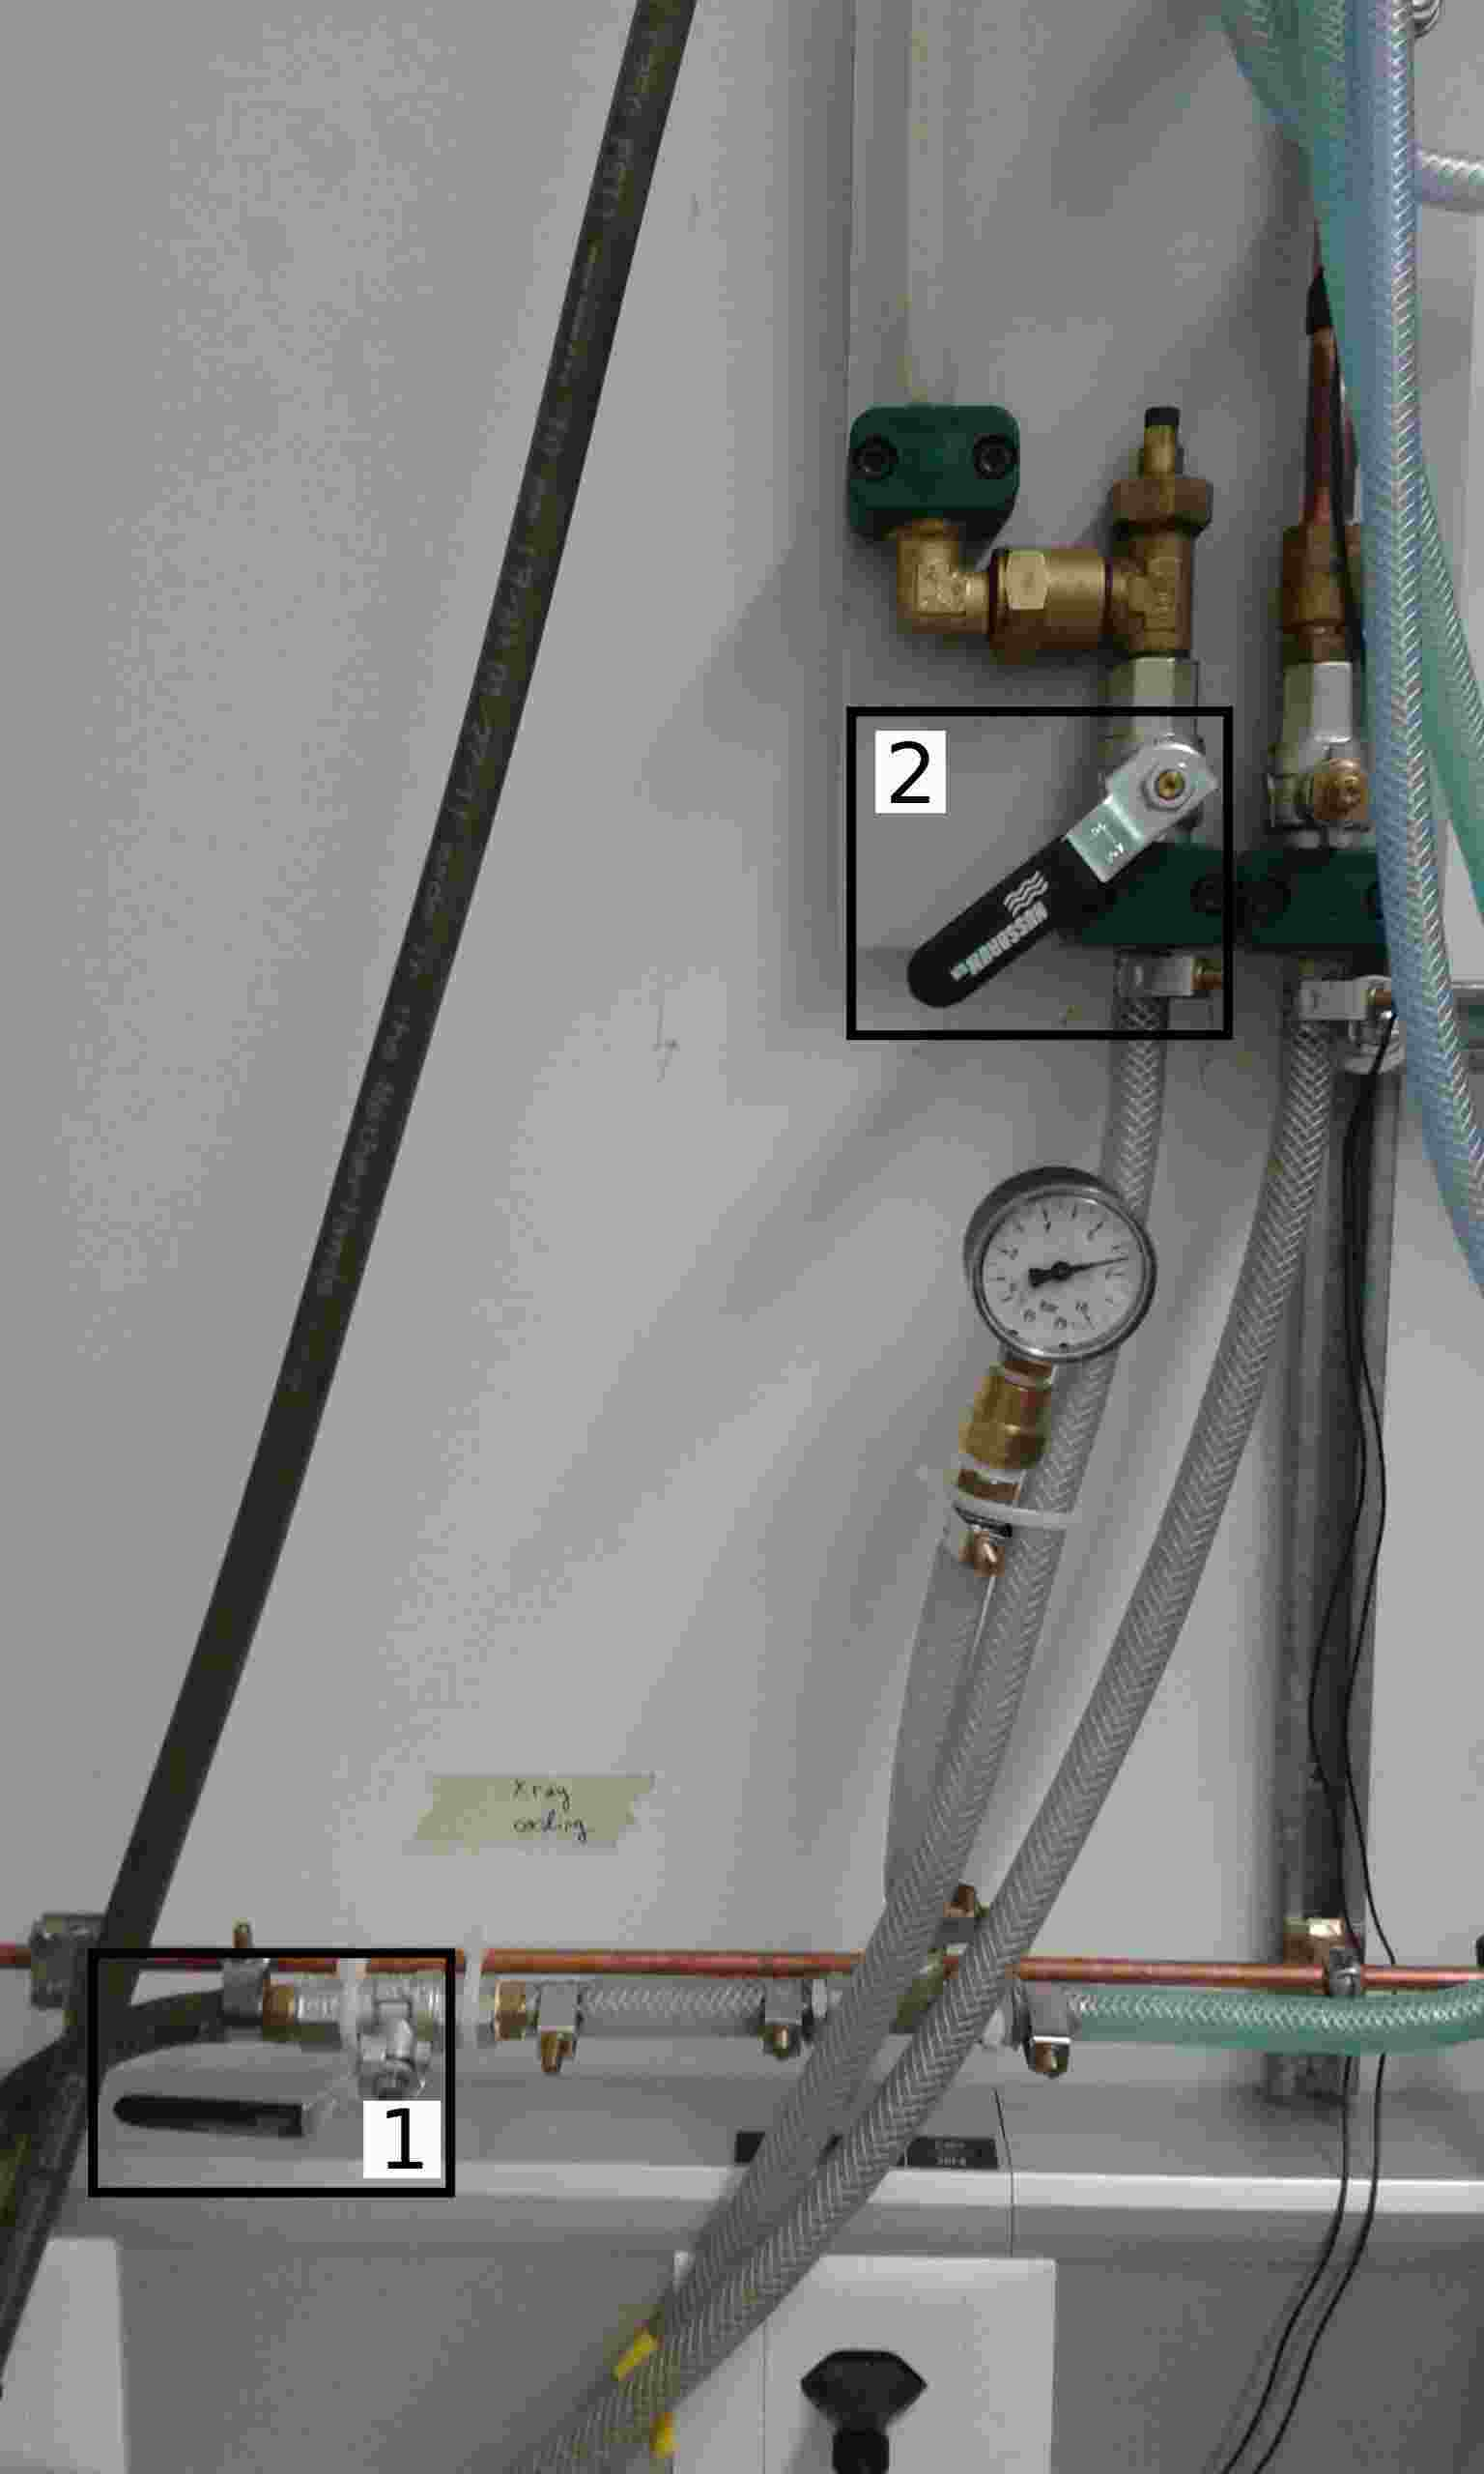
\includegraphics[width=0.3\textwidth, angle=0] {./graphics/Water.jpg}
\end{figure}
}
\item {Switch on X-ray machine (3).
\begin{figure} [h!] \centering 
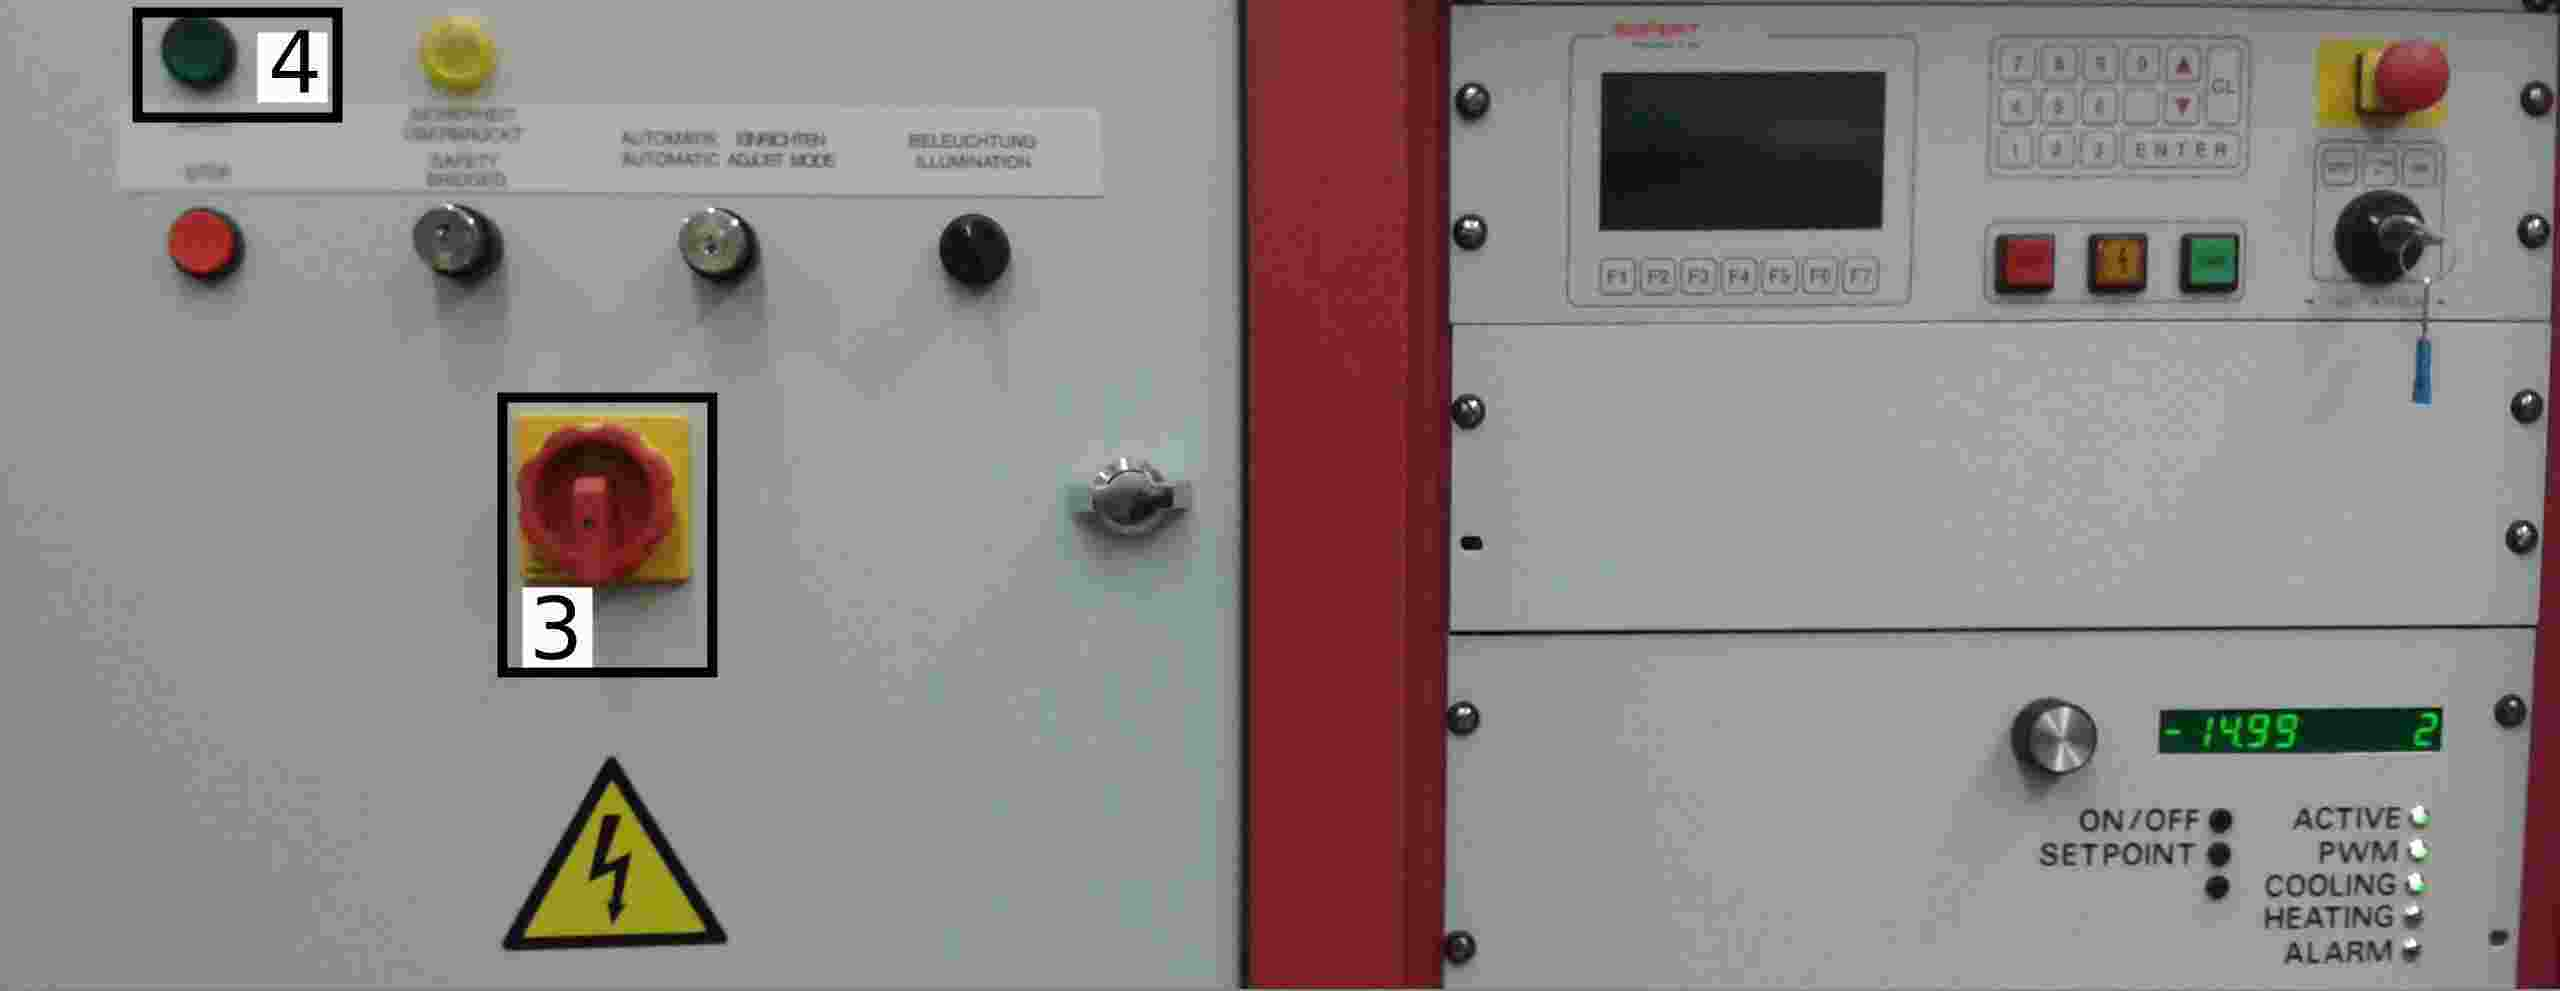
\includegraphics[width=0.4\textwidth, angle=0] {./graphics/Full2.jpg}
\end{figure}
}
\item {(Re)close the door of the X-ray setup housing, press round, green \textbf{START} button (4).}
\item {Turn key to \textbf{ON}.
\begin{figure} [h!] \centering 
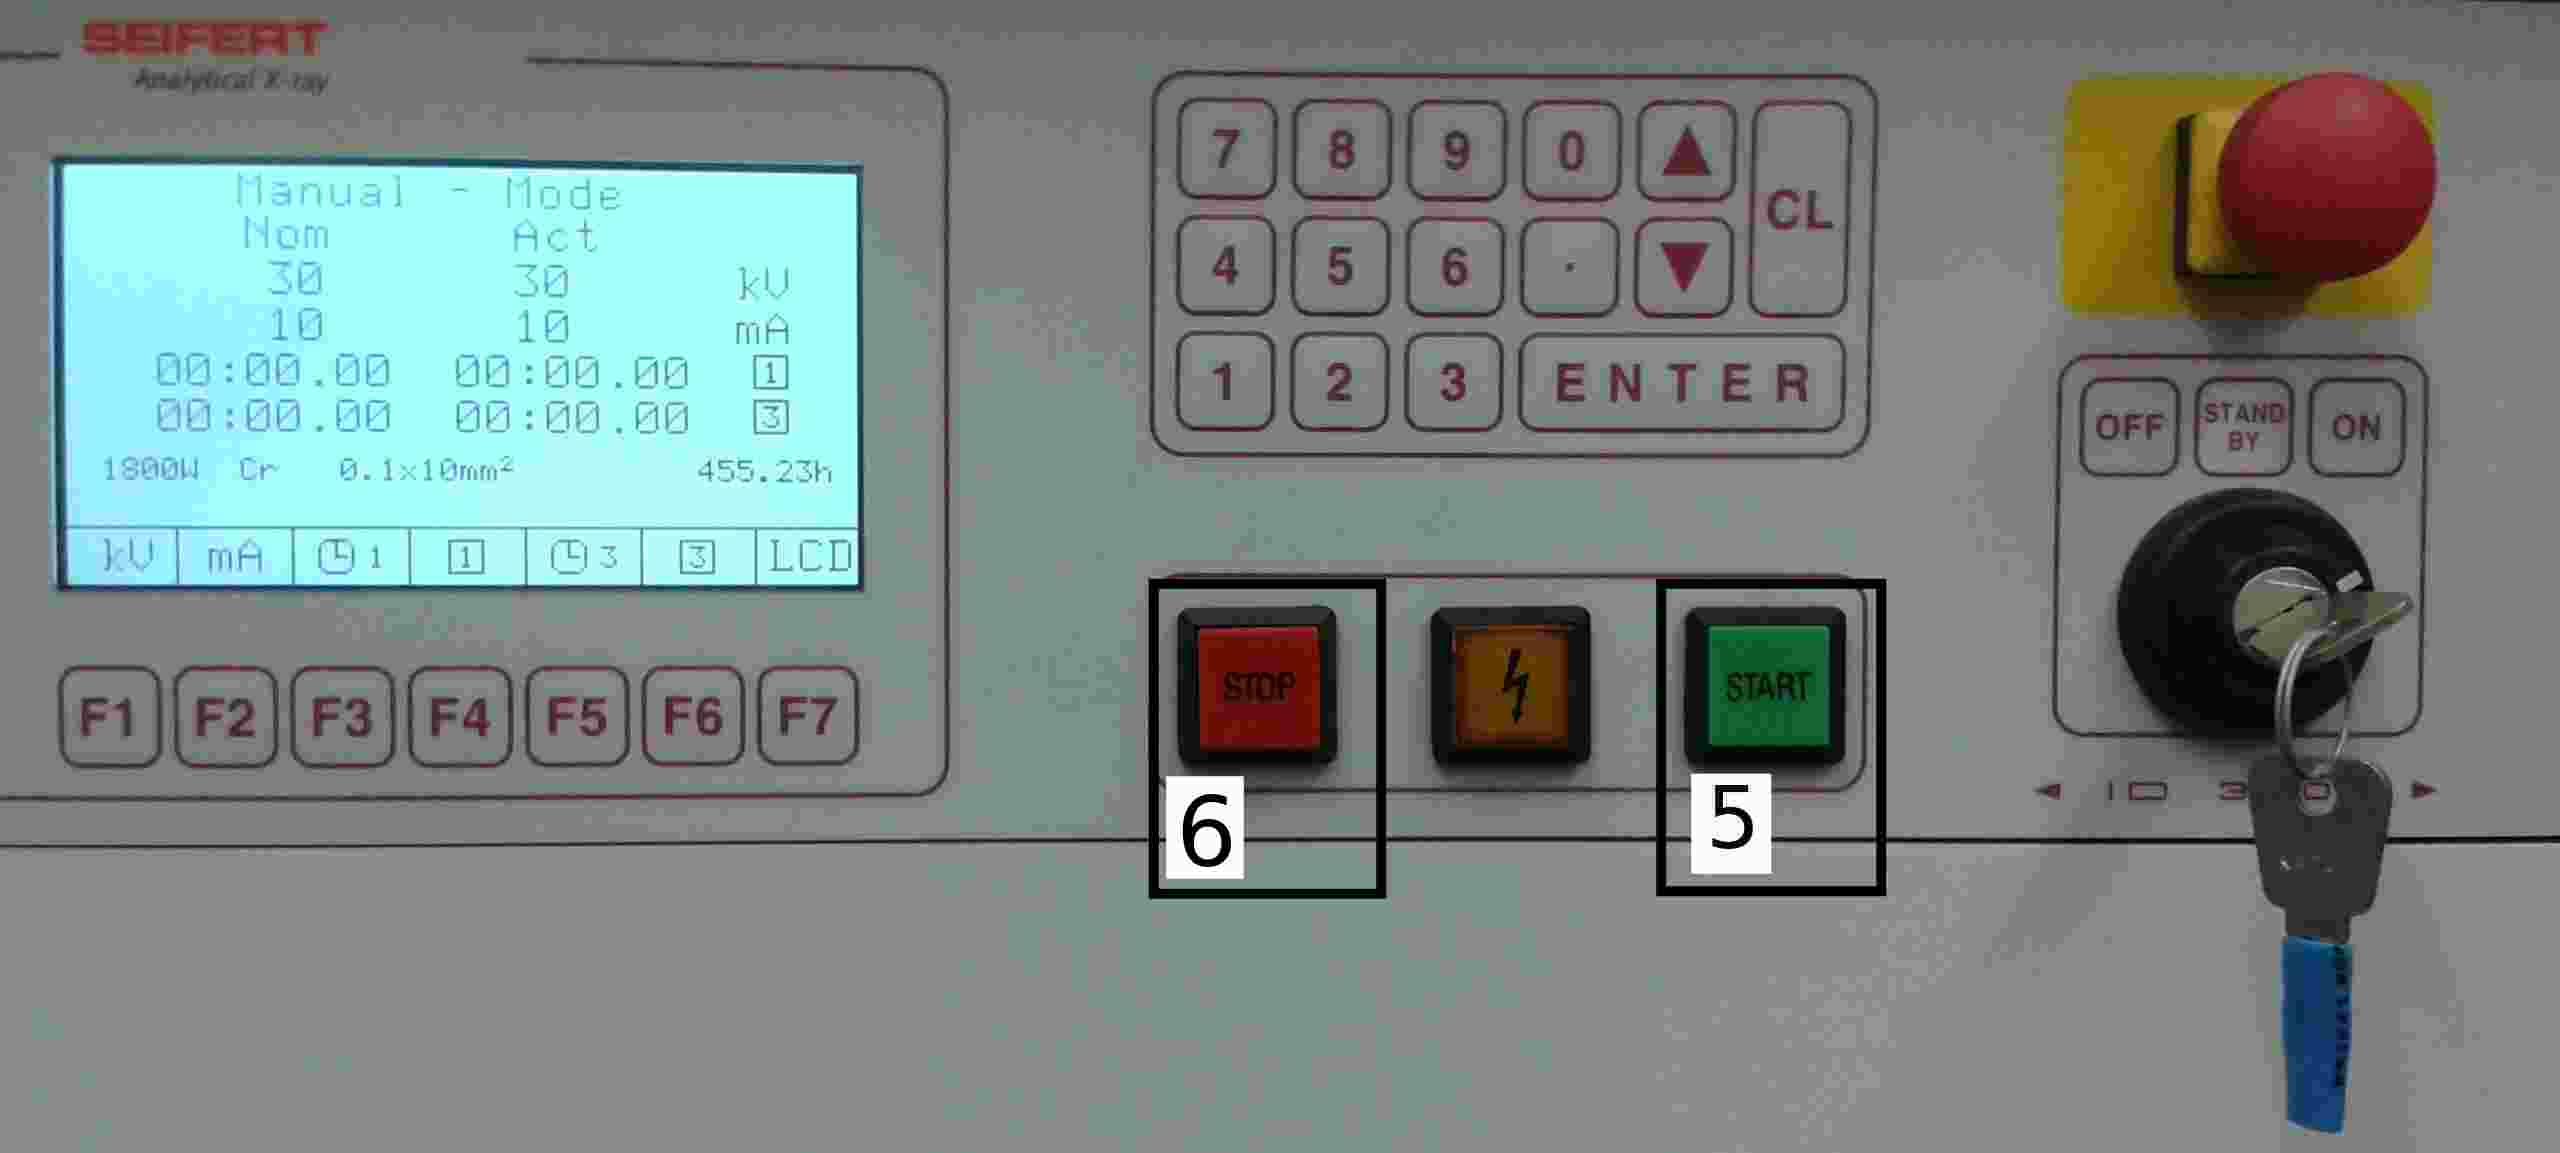
\includegraphics[width=0.4\textwidth, angle=0] {./graphics/CommandBoard2.jpg}
\end{figure}
}
\item{Warm up X-ray tube by selecting \textbf{F7}. Enter the required current and voltage settings by selecting \textbf{F2, F4 or F6}. One shouldn't have very small values for currents with large voltages as well as the other way around. Suggested values are 60 kV and 30 mA for warming up the tube. Press \textbf{Enter} when finished, then \textbf{START} (square green one, 5). This will take up to 30 minutes depending on when the tube was operated the last time at this or a higher voltage. If the voltage is not set, check green interlock button (4) and the door, press \textbf{CL} to delete the error message.}
\item {To control X-ray tube settings and targets during operation, use respectively \textbf{id3003} and \textbf{xrf} programs. Shutter 1 directs the beam to the targets, shutter 3 directs it to the modules. Available targets are Zn, Cu, Mo, Ag, Sn, Ba, Br (Screen). Some examples:
\shellcmd{
id3003.py open shutter 1\\
id3003.py close shutter 1\\
id3003.py set hv on\\
id3003.py set hv off\\
id3003.py set voltage 30\\
id3003.py set current 10\\
id3003.py get voltage\\
id3003.py get current\\
xrf Ag, xrf Mo\\
xrf Screen\\
}
}
\item{When taking a break, turn off high voltage and close the shutter. Turn key to \textbf{STAND BY}.}
\end{itemize}


\section{Set-up parameter directory}

The parameters for the X-ray test are copied from the \testname{FullTest}@17 from the ColdBox.

\begin{itemize}
\item copy coldbox parameter folder \textbf{004\_FulltestPxar\_p17} to /data/moduleParameters, and rename to module name \textbf{Mxxx}
\item either manually delete .root and .log files or (in /data/moduleParameters) use the script \textbf{python ./clean\_parameters\_folder.py -d Mxxx}
\item  (temporary) copy \textbf{testParameters.dat} from /data/moduleParameters/testParameters.dat to \textbf{/data/moduleParameters/Mxxx/testParameters.dat}
\end{itemize}

\section{elComandante configuration}

\begin{itemize}
\item use elComandante from \textbf{/home/production/elComandante{\color{Red} Xray}/}
\item check test chain in .ini file
\item $[Tests]$:\\
{\it {\bf Test} = PixelAlive@17$>$ GainPedestal@17$>$ RetrimHotPixels @150MHz/cm2$>$
HRData@50MHz/cm2, HRData @150MHz/cm2, HRSCurves@100MHz/cm2,
XraySpectrum@Zn, XraySpectrum@Mo, XraySpectrum@Ag, XraySpectrum@Sn,
CalDelScanAndSaveDacs@4mA25kV$>$ HREfficiency@50MHz/cm2,
HREfficiency@100MHz/cm2, HREfficiency@150MHz/cm2,
HREfficiency@200MHz/cm2, HREfficiency@250MHz/cm2\\
{\bf TestDescription} = XrayQualification}
\end{itemize}

%\shellcmd{$[Tests]$
%Test = PixelAlive@17> GainPedestal@17> RetrimHotPixels@150MHz/cm2>
%HRData@50MHz/cm2, HRData@150MHz/cm2, HRSCurves@100MHz/cm2,
%XraySpectrum@Zn, XraySpectrum@Mo, XraySpectrum@Ag, XraySpectrum@Sn,
%CalDelScanAndSaveDacs@4mA25kV> HREfficiency@50MHz/cm2,
%HREfficiency@100MHz/cm2, HREfficiency@150MHz/cm2,
%HREfficiency@200MHz/cm2, HREfficiency@250MHz/cm2
%TestDescription = XrayQualification
%}


\section{Run test}

\begin{itemize}
\item use elComandante from \textbf{/home/production/elComandante{\color{Red} Xray}/elComandante}
\item run ./el\_comandante.py
\item scan modules with scanner from left to right, press enter for an empty position or if the module is the same than in the previous test.
\end{itemize}


\section{After test}

\begin{itemize}
\item check test list in elComandante output (below "Final cleanup after all tests ..."), status code should always be 1. A status code of $\neq 1$ or red color means error
\item copy files from local directory (eg. /usr/local/data/) to /home/production/data, copying .tar files and extracting them is faster.
\item analyze with MoReWeb
\item update MoReWeb overview on our webserver, script \textbf{/home/production/ synchronize\_webserver.sh}
\item write Elog entry
\item upload to database
\item the steps mentioned above are similar to the Cold Box qualification, which is documented in section \ref{postdata}.
\end{itemize}


\section{Switching off X-ray setup}
\begin{itemize}
\item {Close the shutter, turn off high voltage.}
\item {Press \textbf{STOP} (6).}
\item {Turn key to \textbf{OFF}.}
\item {Turn off X-ray machine.}
\item {Close both water valves.}
\end{itemize}

\section{Troubleshooting}

\prob{DTBs are not detected by the computer, typical error message: Unable to detach testboard. Usbview is very slow and might or might not list all connected DTBs}
\sol{Run the script \textbf{/home/production/reset\_usb.sh} (as root) or restart computer (only after agreement from the group).}
\prob{Hot Pixel Re-trimming takes very long or finds more hot pixels than usual}
\sol{Might be missing HV or wrong testParameters.dat file (for instance from an old pXar version)}
\prob{Keithley is not turned on by elComandante}
\sol{check if the \textbf{port} option in section \textbf{keithleyClient} in \textbf{elComandante.conf} is pointing to the correct device. Find the device by running the command \mbox{\textbf{findkeithley}} on production user. This device number can reset after reboot!}
\prob{How to abort the program?}
\sol{In case of emergency, terminate elComandante with Ctrl-C. The data should be stored in /usr/local/coldboxDATA. Then one can turn off the setup as described in section 5.}




%------------------------------------------------
\phantomsection

%\section*{Acknowledgments} % The \section*{} command stops section numbering

%\addcontentsline{toc}{section}{Acknowledgments} % Adds this section to the table of contents



%----------------------------------------------------------------------------------------
%	REFERENCE LIST
%----------------------------------------------------------------------------------------
\phantomsection
\bibliographystyle{unsrt}

%----------------------------------------------------------------------------------------

\end{document}